\chapter{Results}
\label{Chap4}
\section{Powder ageing}

\subsection{Grain size and distribution}
\subsubsection{Fresh powder}

\subsubsection{Recycled powder}
\subsection{Composition}

\subsubsection{Fresh powder}

\subsubsection{Recycled powder}
Faire graphe avec barres d'erreurs
 \begin{center}
\begin{table}[ht]
\noindent\makebox[\textwidth]{\begin{tabular}{|c|c |c |c| c|}
    \hline
    Date of sampling& \multicolumn{4}{c}{Composition [\%wt]} \vline\\
    \cline{2-5}
    & Al& Fe&Mg&Si\\
\hline 
\hline   
    23/10/2017  &89.2&0.12&0.49&10.2\\
    09/01/2018 & 89.3 & 0.13 &0.48&10.1\\
    12/01/2018 & 89.4 & 0.13 &0.48&10\\
    21/02/2018&89.1&0.19&0.51&10.3\\
    13/03/2018 &89.1&0.16&0.51&10.1\\    
    \hline
\end{tabular}}

\caption[Composition of recycled AlSi10Mg powder as a function of the date]{Composition of recycled AlSi10Mg powder as a function of the date}
\label{tab:compo}
\end{table}
 \end{center}

\section{Density and hardness study}
\subsection{Optimisation of the SLM parameters}
\label{Rparaopti}
The optimisation of the manufactured samples properties was done with respect to $\rho_{a,rel}$ and $H_v$. For this purpose, twelve cubes were fabricated with P varying from 0.75\% $P_{max} $to $P_{max}$ and $v_s$ from 900 to 1500 [$\frac{mm}{sec}$]. Details about batch X200-171024 are given in appendix \ref{AppendixA}. The goal of this optimisation was to select a single set of parameters values to use in the rest of the thesis. The parameters values were chosen to cover a wide range of $E_d$. Sets of parameters ($P=75\% P_{max}$ ; $v_s=1200 [\frac{mm}{sec}]$) and ($P=75\% P_{max}$ ; $v_s=900 [\frac{mm}{sec}]$) gave the best results in terms of $\rho_{a,rel}$ in a previous study done at UCL. It was decided to produce samples with these sets of values in triplicate in order to have a first insight on the process reproducibility. This will be discussed further in next section. Here, only the mean $H_v$ and $\rho_{a,rel}$ of those samples will be compared to the others'.\\

Results for the measurements of $\rho_{a,rel}$ and $H_v$ are summarised in figure \ref{fig:HD2-171024} and detailed in appendix \ref{AppendixA}. The 95\% confidence intervals (CI) are drawn on the graphs. The methods used to compute them are described in appendix \ref{AppendixC}. All apparent relative density values were obtained through hydrostatic weighing of the unpolished AB specimens.\\

\begin{figure}[ht]
\centering
\noindent\makebox[\textwidth]{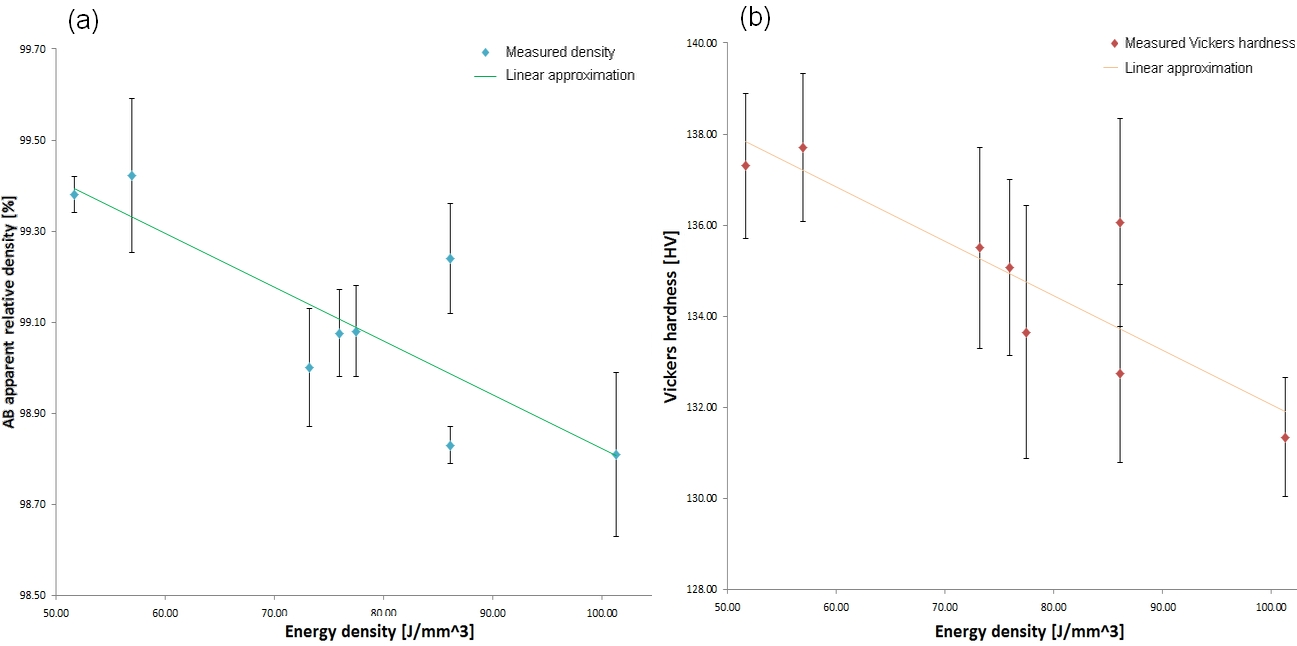
\includegraphics[scale=0.5]{Images/HD2-171024}}
\decoRule
\caption[Batch X200-171024 samples properties as a function of the energy density: (a) as-built apparent relative density (b) Vickers hardness]{Batch X200-171024 samples properties as a function of the energy density: (a) as-built apparent relative density (b) Vickers hardness}
\label{fig:HD2-171024}
\end{figure} 

 The graph shows a general progressive decrease of  $\rho_{a,rel}$ and $H_v$ for $E_d>57 [\frac{J}{mm^3}]$.


\subsection{Reproducibility}
\label{RReprod}
%\subsubsection{Relative density and hardness}
\subsubsection{General results}
Following the optimisation of the set values (see section \ref{Rparaopti}), it was decided to produce a batch of fifteen type "7" cubic samples and fifteen others of type "8" in order to assess the process reproducibility when using a same powder. The two sets of parameters were used to compare the results for optimal and sub-optimal set values. A total of 18 samples were fabricated close to one another (see \ref{fig:180109-real}) to see if the specimens rapprochement has any effect on their final properties. The apparent relative density was once more measured with the unpolished AB samples.\\

Hardness and apparent relative density results are shown on figure \ref{fig:HD-171024}. The key information is displayed in tables \ref{tab:78b} and \ref{tab:78bb}. Type "8" samples exhibited slightly poorer properties than type "7" ones in average. However, the former have far better properties to what one could have expected based on previous results (see table \ref{tab:78}). The highest measured density is 99.54 [\%].\\

\begin{figure}[ht]
\centering
\centerline{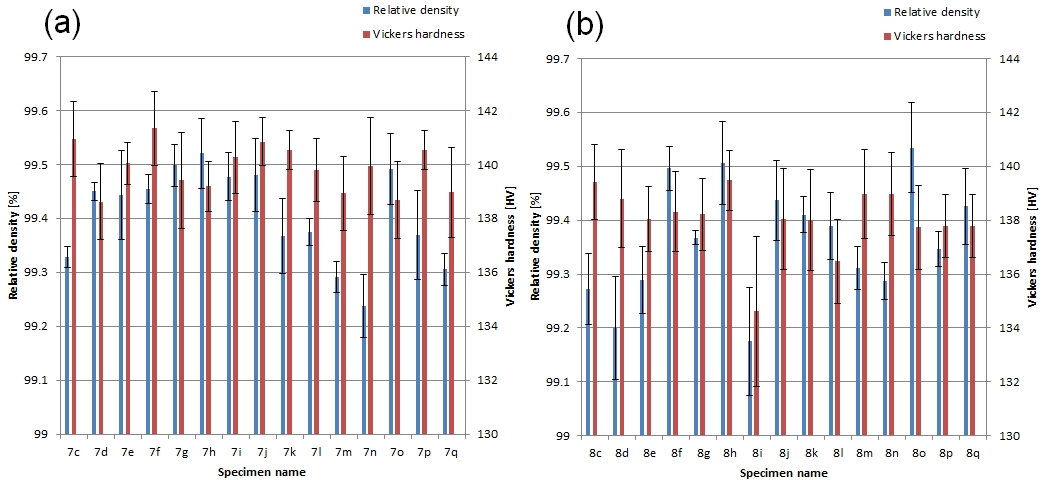
\includegraphics[scale=0.65]{Images/HD-180109-both}}
\decoRule
\caption[As-built apparent relative density and hardness results of batch X200-180109 for (a) type "7" samples (b) type "8" samples.]{As-built apparent relative density and hardness results of batch X200-180109 for (a) type "7" samples (b) type "8" samples.}
\label{fig:HD-171024}
\end{figure} 

 \begin{center}
\begin{table}[ht]
\noindent\makebox[\textwidth]{\begin{tabular}{|c|c|c |c |c|}
    \hline
    Type & $\overline{\rho_{a,rel}}$ [\%] & $SD_{\rho_{a,rel}}$[\%]& $\overline{H_v}$ [HV]& $SD_{H_v}$[HV]\\

\hline
\hline   
    7 & 99.42 & 0.08 & 138 & 0.4 \\
    8 & 99.08 & 0.27 & 135 & 1.3 \\
\hline

\end{tabular}}

\caption[Standard deviations and average values for apparent relative densities and hardnesses of types "7" and "8" specimens of batch X200-171024]{Standard deviations and average values for apparent relative densities and hardnesses of types "7" and "8" specimens of batch X200-171024}
\label{tab:78}
\end{table}
 \end{center}

 \begin{center}
\begin{table}[ht]
\noindent\makebox[\textwidth]{\begin{tabular}{|c|c|c |c |c|}
    \hline
    Type & $\overline{\rho_{a,rel}}$ [\%] & $SD_{\rho_{a,rel}}$[\%]& $\overline{H_v}$ [HV]& $SD_{H_v}$[HV]\\

\hline
\hline   
    7 & 99.40 & 0.09 & 139.9 & 0.87 \\
    8 & 99.36 & 0.11 & 138.3 & 1.3 \\


\hline
\end{tabular}}

\caption[Standard deviations and average values for apparent relative densities and hardnesses of types "7" and "8" specimens of batch X200-180109]{Standard deviations and average values for apparent relative densities and hardnesses of types "7" and "8" specimens of batch X200-180109}
\label{tab:78b}
\end{table}
 \end{center}
 
 
 \begin{center}
\begin{table}[ht]
\noindent\makebox[\textwidth]{\begin{tabular}{|c|c|c |c |c|}
    \hline
    Type & $min(\rho_{a,rel})$ [\%] & $max(\rho_{a,rel})$[\%]& $ min(H_v)$ [HV]& $min(H_v)$[HV]\\

\hline
\hline   
    7 & 99.24 & 99.52 & 138.6 & 141.4 \\
    8 & 99.18 & 99.54 & 134.6 & 140.4 \\


\hline
\end{tabular}}

\caption[Minimal and maximal values for apparent relative densities and hardnesses of types "7" and "8" specimens of batch X200-180109]{Minimal and maximal values for apparent relative densities and hardnesses of types "7" and "8" specimens of batch X200-180109}
\label{tab:78bb}
\end{table}
 \end{center}

\subsubsection{Sample proximity and position influence}
The results where displayed in figure \ref{fig:180109-HD} as functions of the (x,y) positions of the samples on the manufacturing plate. The coordinated are such that the roll sweeps were done in the positive $x$ direction during the fabrication. Other graphs showing the averaged $\rho_{a,rel}$ and $H_v$ as functions of the x and y coordinates were also plotted. To do so, the samples distanced from less than 1 [cm] along x or y were considered to have the same corresponding coordinate. The graphs are shown in appendix \ref{AppendixD}.\\
\begin{figure}[ht]
\centering
\centerline{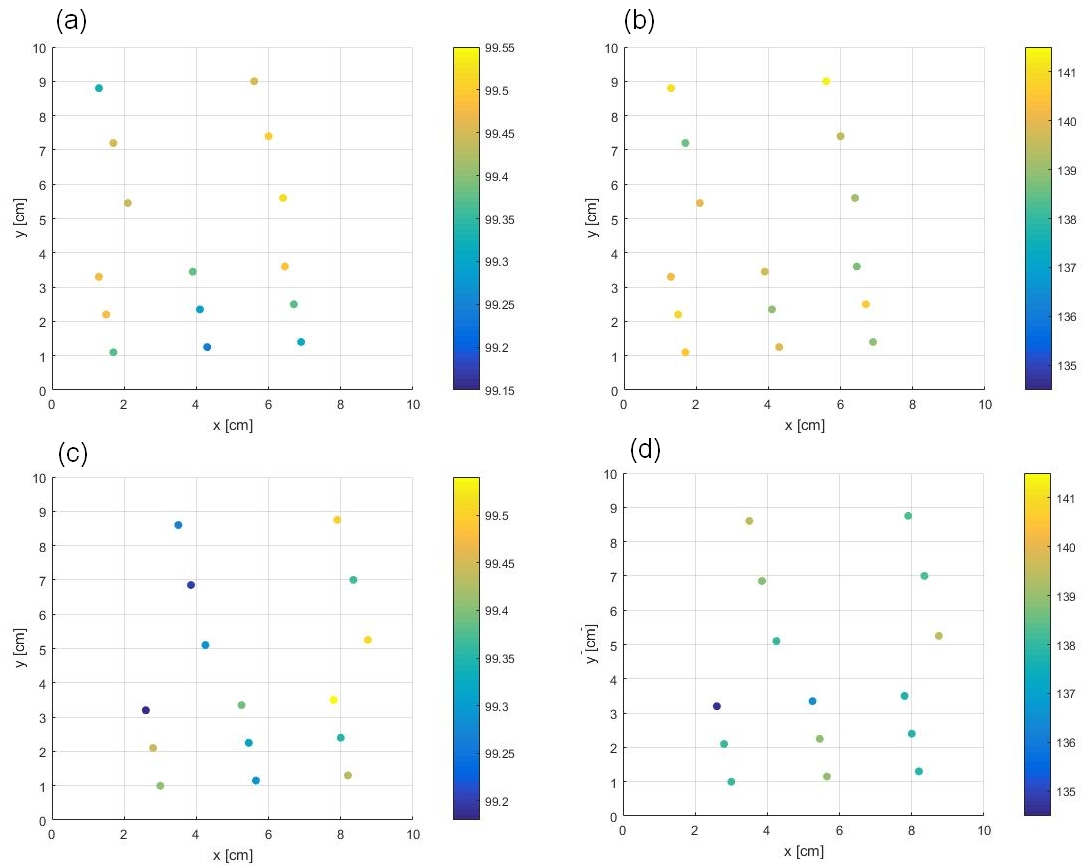
\includegraphics[scale=0.62]{Images/180109-HD}}
\decoRule
\caption[Batch X200-180109 scatter plots as functions of the (x,y) position on the manufacturing plate: (a) type "7" apparent relative densities (b) type "7" hardnesses (c) type "8" apparent relative densities (d) type "8" hardnesses]{Batch X200-180109 scatter plots as functions of the (x,y) position on the manufacturing plate: (a) type "7" apparent relative densities (b) type "7" hardnesses (c) type "8" apparent relative densities (d) type "8" hardnesses}
\label{fig:180109-HD}
\end{figure} 

Effets proximités, tendances selon x et y..........................\\
\subsubsection{Scan order influence}


\begin{figure}[ht]
\centering
\centerline{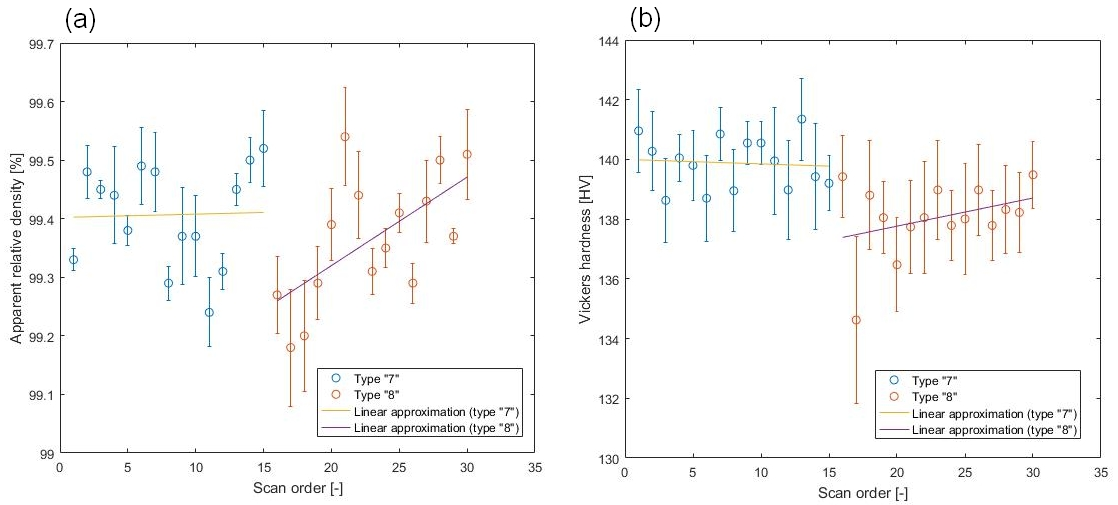
\includegraphics[scale=0.62]{Images/180109-SO}}
\decoRule
\caption[Batch X200-180109 scatter plots as functions of the scan order of (a) the apparent relative densities (b) the Vickers hardnesses]{Batch X200-180109 scatter plots as functions of the scan order of (a) the apparent relative densities (b) the Vickers hardnesses}
\label{fig:180109-SO}
\end{figure} 

\subsection{Homogeneity}
As said in section \ref{MMFPP}, all tensile specimens were fabricated vertically. Their height is significantly greater than the other samples'; respectively 6 [cm], and 1 [cm] or less. It was chosen to cut up specimen X200-180417-25 into slices to measure if the density and hardness were homogeneous along the Z direction in the material. The surfaces analysed were named according to their original Z position in the specimen with "B", "C1" , "C2", "C3" and "T" (for bottom, center and top) and to the test done with a letter "D" or "H"  (for density and hardness). The denomination is summarised in figure \ref{fig:saus}.\\

\begin{figure}[ht]
\centering
\centerline{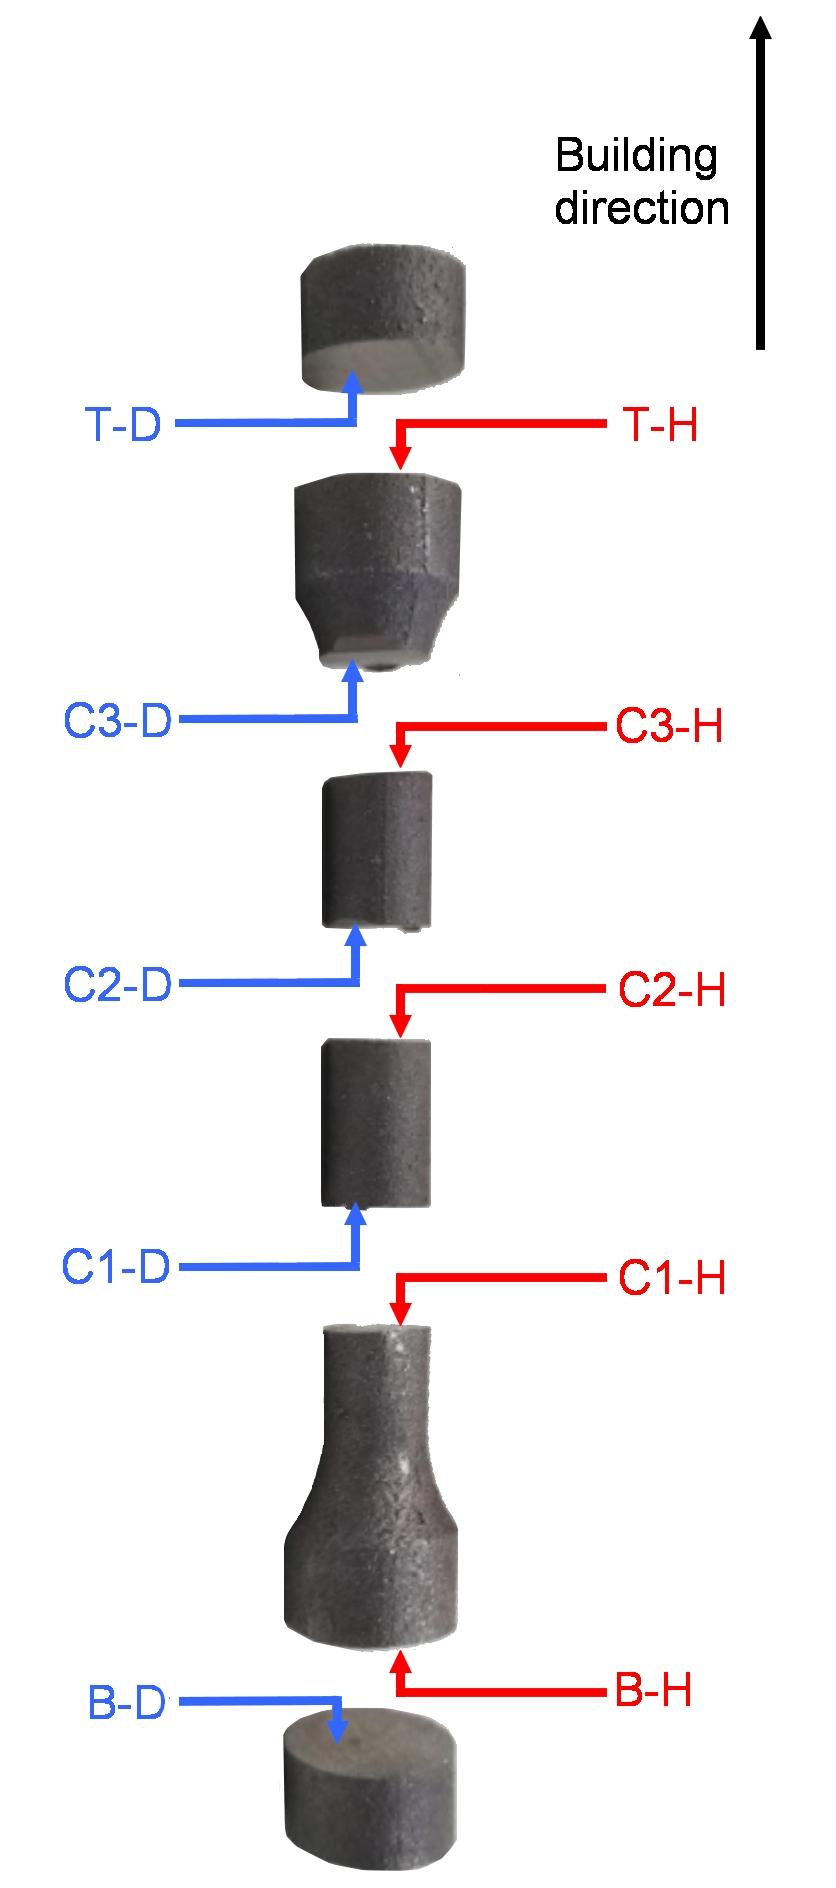
\includegraphics[scale=0.23]{Images/Saus}}
\decoRule
\caption[Specimen X200-180417-25 sub-parts and surfaces denomination]{Specimen X200-180417-25 sub-parts and surfaces denomination.}
\label{fig:saus}
\end{figure}

Results are shown in figure \ref{fig:HD-180417}. With regard to hardness, no general trend could be observed. The measured values are high and closely packed except for the "B" surface, which exhibited a significantly lower hardness. Density values are all equal or above 99.75 [\%]. The values at the center of the sample were slightly lower to the extremities'. A summary of the results is displayed in table \ref{tab:25}.

 \begin{center}
	\begin{table}[ht]
		\begin{tabular}{|c|c |c |c| c|}
			\hline
			Property& Average value & Minimum & Maximum & Standard deviation \\
			\hline 
			\hline   
			Relative density [\%] & 99.80 & 99.75 & 99.87 & 0.05\\
			Hardness [HV] &138.0 &132.2 &141.7&3.5\\
			\hline
		\end{tabular}

		\caption[Relative density and hardness results summary for specimen X200-180417-25 surfaces]{Relative density and hardness results summary for specimen X200-180417-25 surfaces}
		\label{tab:25}
	\end{table}
\end{center}


\begin{figure}[ht]
\centering
\centerline{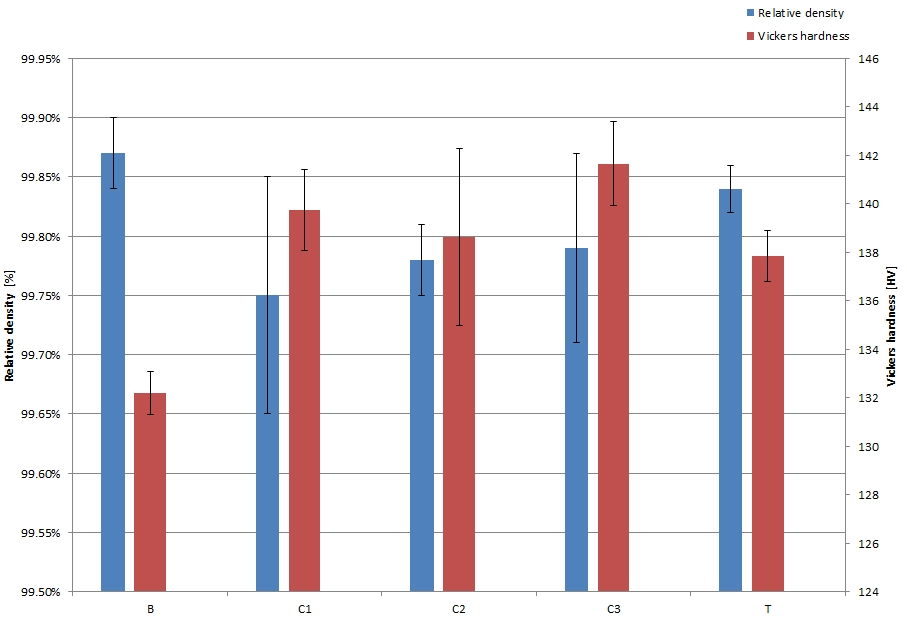
\includegraphics[scale=0.62]{Images/HD-180417}}
\decoRule
\caption[RODIA based relative density and hardness results for specimen X200-180417-25 surfaces]{RODIA based relative density and hardness results for specimen X200-180417-25 surfaces}
\label{fig:HD-180417}
\end{figure} 

\section{Characterisation of the as-built samples} 
\label{RCABS}
\subsection{Melt pools sizes and distribution}

\subsection{Microstructure}


\subsection{Residual stresses}

\subsection{Mechanical properties}

The average tensile properties of the as-built specimens are displayed in table \ref{tab:tracMAB}. Detailed information may be consulted in appendice \ref{AppendixAbis}. Very similar behaviours were observed for samples with and without contour scanning strategy. No distinction shall thus be made between the two in what follows. [Critère de considère]
 \begin{center}
\begin{table}[ht]
\noindent\makebox[\textwidth]{\begin{tabular}{|c |c |c| c|}
    \hline
     E [GPa] & $\sigma_y$ [MPa] & $\sigma_u$ [MPa] & $\epsilon_f$[\%] \\

\hline
\hline   
    64.9 $\pm 3.0$ & 266.6 $\pm 23.6$ & 381.7 $\pm 24.7$ & 2.5 $\pm 0.5$  \\

    \hline
\end{tabular}}

\caption[Average tensile mechanical properties of the as-built specimens from batch X200-180417]{Average tensile mechanical properties of the as-built specimens from batch X200-180417}
\label{tab:tracMAB}
\end{table}
 \end{center}
\section{Characterisation of the heat-treated samples}
\label{RCHTS}
\subsection{Microstructure}

 
\subsection{Residual stresses}

\subsection{Mechanical properties}

Parler de RAMBERG-OSGOOD

 \begin{center}
\begin{table}[ht]
\noindent\makebox[\textwidth]{\begin{tabular}{|c|c |c |c| c|c|}
    \hline
     HT & E [GPa] & $\sigma_y$ [MPa] & $\sigma_u$ [MPa] & $\epsilon_{f,eng}$[\%] & $\epsilon_{f,true}$ [\%] \\

\hline
\hline   
   150$^\circ$C (2h) & 68.4 $\pm 1.9$ & 288.2 $\pm 1.4$ & 441.7 $\pm 5.5$ & 5.5 $\pm 0.8$&-  \\
    200$^\circ$C (2h) &  72.1 $\pm 0.4$ & 245.4 $\pm 0.6$ & 382.0 $\pm 11.4$ & 4.6 $\pm 0.3$ &- \\
     250$^\circ$C (2h) &  70.6 $\pm 1.0$ & 235.1 $\pm 7.4$ & 340.9 $\pm 12.2$ &8.8 $\pm 0.2$ & 16.5 $\pm 0.1$  \\
      300$^\circ$C (2h) &  68.9 $\pm 0.6$ & 170.7 $\pm 1.7$ & 252.9 $\pm 10.4$ &13.6 $\pm 0.5$ & 29.7 $\pm 0.1$  \\

    \hline
\end{tabular}}

\caption[Average tensile mechanical properties of the heat-treated specimens from batch X200-180417]{Average tensile mechanical properties of the heat-treated specimens from batch X200-180417}
\label{tab:tracMAB}
\end{table}
 \end{center}

\begin{figure}[ht]
\centering
\centerline{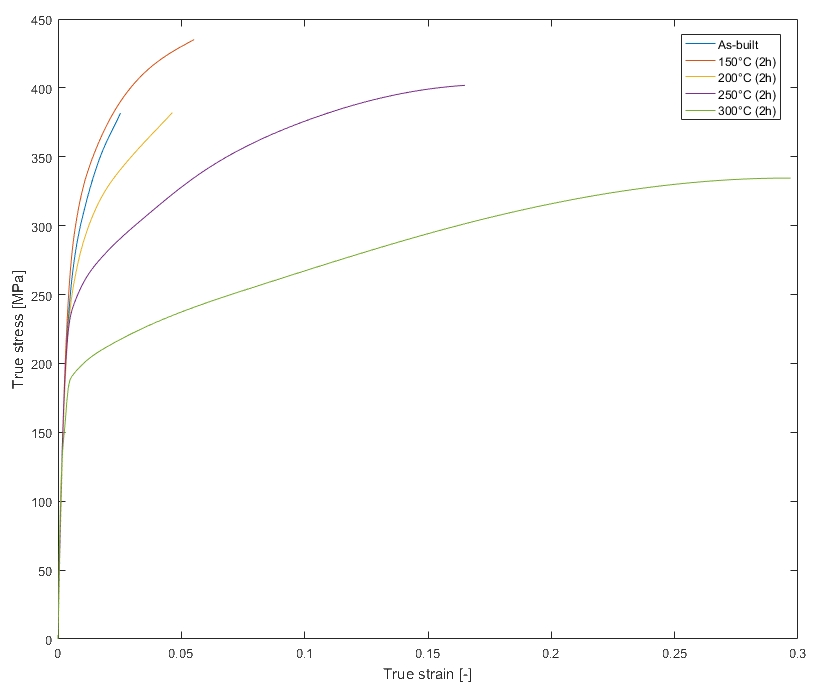
\includegraphics[scale=0.23]{Images/MeanTrac}}
\decoRule
\caption[Average stress-strain curves of the tensile specimens of batch X200-180417.]{Average stress-strain curves of the tensile specimens of batch X200-180417.}
\label{fig:MeanTrac}
\end{figure}

%\begin{table}
%\caption{The effects of treatments X and Y on the four groups studied.}
%\label{tab:treatments}
%\centering
%\begin{tabular}{l l l}
%\toprule
%\tabhead{Groups} & \tabhead{Treatment X} & \tabhead{Treatment Y} \\
%\midrule
%1 & 0.2 & 0.8\\
%2 & 0.17 & 0.7\\
%3 & 0.24 & 0.75\\
%4 & 0.68 & 0.3\\
%\bottomrule\\
%\end{tabular}
%\end{table}